\subsection{整元的范数与迹}

命题 17. 设 A 是环，B 是（交换）A-代数，X 是 B 上的 n 阶方阵；则下列性质等价：

\begin{enumerate}
\def\labelenumi{(\alph{enumi})}
\item
  \(X\) 在 A 上是整的。
\item
  存在 \(\mathbf{M}\) （\(\mathbf{B}^n\) 的一个有限生成子 A-模），使得 \(X.x\in \mathbf{M}\) 对所有 \(x\in \mathbf{M}\) 成立，且 \(\mathbf{M}\) 是 B-模 \(\mathbf{B}^n\) 的一个生成系。
\item
  \(X\) 的特征多项式的系数在 \(\mathbf{A}\) 上是整的。
\end{enumerate}

  若 \(\chi(T) = \det(T.1 - X)\) 是 \(X\) 的特征多项式，则 Cayley-Hamilton 定理表明 \(\chi(X) = 0\)（《代数》第 VII 章，§ 5，第 4 节，注 1），且由于 \(\chi\) 是首一多项式，由第 1 节命题 6 知 (c) 蕴含 (a)。

  其次假设 (a) 成立。若 \((e_i)_{1 \leqslant i \leqslant n}\) 是 \(B^n\) 的典范基，则由诸 \(X^k \cdot e_i\)（ \(1 \leqslant i \leqslant n, k \geqslant 0\) ）生成的 B 的子 A-模 M 是有限生成 A-模，因为 A-代数 A[X] 是有限生成 A-模（第 1 节，定理 1）；由于 M 包含诸 \(e_i\) ，可见 (a) 蕴含 (b)；其逆是第 1 节定理 1 条件 \((E_{\mathrm{III}})\) 的推论。

  最后证明 (a) 蕴含 (c)；由于 X 在 A 上整，从而更加在多项式环 A[T] 上整，故 T.1 - X 也在 A[T] 上整，且由第 3 节命题 12 可见，问题可化归（把 X 换成 T.1 - X，把 A 换成 A[T]）为证明：若 X 在 A 上整，则 \(d = \det(X)\) 是 B 中在 A 上整的元素。而上面已经看到，由 X 定义的 \(B^{n}\) 的自同态 u 使一个包含诸 \(e_{i}\) 的有限生成子 A-模 M 保持稳定；于是 n-向量 \(x_{1} \wedge x_{2} \wedge \cdots \wedge x_{n}\) ，其中 \(x_{i} \in M\)

（ \(1 \leqslant i \leqslant n\) ）的这些向量于是在 \(\bigwedge (\mathbf{B}^n)\) 中生成一个包含 \(e_1 \wedge e_2 \wedge \cdots \wedge e_n\) 的有限生成子 A-模，它在 \(\bigwedge^n u\) 之下稳定，换言之在比率为 \(d\) 的位似之下稳定；由于

\[
e _ {1} \wedge e _ {2} \wedge \dots \wedge e _ {n}
\]

在 B 中的零化子仅为 0，故第 1 节定理 1 的条件 \((\mathbf{E}_{\mathrm{III}})\) 证明 \(d\) 在 A 上是整的。

推论 1. 设 A 是整环，K 是它的分式域，K' 是有限维 K-代数（不一定交换）。若 \(x \in \mathbf{K}'\) 在 A 上是整的，则特征多项式 \(\mathrm{Pc}_{\mathbf{K}' / \mathbf{K}}(x; \mathbf{X})\)（《代数》第 VIII 章，§ 12，第 2 节）的系数在 A 上是整的。

若 \(z \mapsto M(z)\) 是代数 \(\mathbf{K}'\) 的正则表示（看作矩阵表示；参见《代数》第 VIII 章，§ 13），则 \(\mathrm{Pc}_{\mathbf{K}' / \mathbf{K}}(x; \mathbf{X})\) 按定义就是矩阵 \(M(x)\) 的特征多项式；若 \(x\) 在 \(\mathbf{A}\) 上是整的，则矩阵 \(M(x)\) 在 \(\mathbf{A}\) 上是整的（第 1 节，命题 2），故只需应用命题 17。

推论 2. 在与推论 1 相同的假设与记号下，\(\mathrm{Tr}_{\mathbf{K}^{\prime}/\mathbf{K}}(x)\) 与 \(\mathbf{N}_{\mathbf{K}^{\prime}/\mathbf{K}}(x)\) 都在 A 上是整的。

\(\mathrm{Tr}_{\mathbf{K}^{\prime}/\mathbf{K}}(x)\) 与 \(\mathrm{N}_{\mathbf{K}^{\prime}/\mathbf{K}}(x)\) 是 \(\mathrm{Pc}_{\mathbf{K}^{\prime}/\mathbf{K}}(x;\mathbf{X})\) 的系数（《代数》第 VIII 章，§ 12，第 1 节，公式 (4)），至多相差一个符号，从而是整的。

注 (1) 若 \(\mathbf{K}'\) 是 \(\mathbf{K}\) 上的中心单代数，且 \(x \in \mathbf{K}'\) 在 \(\mathbf{A}\) 上是整的，则 \(x\) 的约化特征多项式（《代数》第 VIII 章，§ 12，第 3 节）的系数在 \(\mathbf{A}\) 上是整的。因为这个多项式有一个方幂等于 \(\mathrm{Pc}_{\mathbf{K}' / \mathbf{K}}(x; \mathbf{X})\)（同前，命题 8），故只需应用命题 17 及第 3 节命题 11。

命题 18. 设 A 是整闭整环，K 是它的分式域，K' 是有限维可分 K-代数（《代数》第 VIII 章，§7，第 5 节），A' 是 A 在 K' 中的整闭包。则 A' 包含在一个有限生成 A-模之中。

该命题可由下面更精确的引理得出：

引理 3. 在命题 18 的假设下，设 \((w_{1},\ldots ,w_{n})\) 是 \(\mathbf{K}'\) 在 \(\mathbf{K}\) 上的包含在 \(\mathbf{A}'\) 中的一组基（第 5 节，命题 16 的推论 2）；则存在唯一的一组基 \((w_{1}^{*},\dots ,w_{n}^{*})\) （\(\mathbf{K}'\) 在 \(\mathbf{K}\) 上的基），使得 \(\mathrm{Tr}_{\mathbf{K}' / \mathbf{K}}(w_i w_j^*) = \delta_{ij}\) （Kronecker 指标）；若 \(d = \mathrm{D}_{\mathbf{K}' / \mathbf{K}}(w_1,\dots ,w_n)\) 是基 \((w_{1},\dots ,w_{n})\) 的判别式（《代数》第 IX 章，§ 2），则 \(d\neq 0\) ，且

\[
\sum_ {i = 1} ^ {n} \mathrm{A} w _ {i} \subset \mathrm{A} ^ {\prime} \subset \sum_ {i = 1} ^ {n} \mathrm{A} w _ {i} ^ {*} \subset d ^ {- 1} \left(\sum_ {i = 1} ^ {n} \mathrm{A} w _ {i}\right).\tag{2}
\]

特别地，若 \(d\) 是 \(\mathbf{A}\) 的可逆元，则 \(\mathbf{A}'\) 是自由 \(\mathbf{A}\) -模，以 \((w_1, \ldots, w_n)\) 为基。

由于 \(\mathbf{K}'\) 是可分 K-代数，故 \(d \neq 0\)（《代数》第 IX 章，§2，命题 5），且 K-双线性形式

\[
(x, y) \mapsto \operatorname{Tr} _ {\mathbf {K} ^ {\prime} / \mathbf {K}} (x y)
\]

在 \(\mathbf{K}'\) 上是非退化的（同前，命题 4）；这就表明了基 \((w_{i}^{*})_{1\leqslant i\leqslant n}\) 的存在性与唯一性（《代数》第 IX 章，§1，第 6 节，命题 6 的推论）。在这样的约定下，(2) 的第一个包含关系是

显然的。设 \(x\) 是 \(\mathbf{A}'\) 的元素；记 \(x = \sum_{i=1} \xi_i w_i^*\) ，其中 \(\xi_i \in \mathbf{K}\) ；对每个 \(i\) ，\(\xi_i = \mathrm{Tr}_{\mathbf{K}' / \mathbf{K}}(xw_i)\) ，故 \(\xi_i\) 在 \(\mathbf{A}\) 上是整的（命题 17 的推论 2），且由于 \(\mathbf{A}\) 是整闭的，有 \(\xi_i \in \mathbf{A}\) （\(1 \leqslant i \leqslant n\)） ；这就证明了第二个

包含关系 (2)。最后，记 \(w_{j}^{*} = \sum_{l=1}^{n} \alpha_{jl} w_{l}\) ，其中 \(\alpha_{jl} \in \mathbf{K}\) ；则 \(\sum_{i=1}^{n} \alpha_{ji} \mathrm{Tr}_{\mathbf{K}'/\mathbf{K}}(w_i w_k) = \delta_{jk}\) 对所有 \(j\) 与 \(k\) 成立；Cramer 公式表明诸 \(\alpha_{ji}\) 属于 \(d^{-1}\mathbf{A}\) ，由此得第三个包含关系 (2)。最后的断言由 (2) 立即得出，因为在此情形 (2) 给出 \(\mathbf{A}' = \sum_{i=1}^{n} \mathbf{A}w_i\) 。

在下面两个推论中，假设与记号均取命题 18 者。

推论 1. 若 A 是 Noether 环，则 A-模 A' 是有限生成的，特别地，环 A' 是 Noether 环。

A' 是一个有限生成 A-模的子模。

推论 2. 若 A 是主理想整环，则 A' 是秩为 n 的自由 A-模。此时自由 A-模的每个子模都是自由的（《代数》第 VII 章，§ 3，定理 1）。

推论 3. 设 E 是有理数域 Q 的 n 次扩张。有理整数环 Z 在 E 中的整闭包的加法群是秩为 n 的自由交换群。

Z 是整闭的（第 3 节，命题 10），且由于 Q 的特征为 0，E 是可分的。因此推论 2 可以应用于 A = Z，K = Q，K' = E 的情形。

注 (2). 若不假设 \(\mathbf{K}'\) 在 \(\mathbf{K}\) 上可分，则推论 1 的结论不一定成立，即使 \(\mathbf{K}'\) 是 \(\mathbf{K}\) 的扩域（习题 20）也是如此。另一方面，若 \(\mathbf{A}\) 是有限生成的整 \(\mathbf{K}_0\) -代数，其中 \(\mathbf{K}_0\) 是域，则正如我们将在 §3 第 2 节定理 2 中看到的，\(\mathbf{A}\) 在其分式域的任意有限次扩张中的整闭包是有限生成 \(\mathbf{A}\) -模，并且是 Noether 环。

\pandocbounded{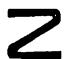
\includegraphics[keepaspectratio]{images/part002_ebb97593.jpg}}

